%%%%%%%%%%%%%%%%%%%%%%%%%%%%%%%%%%%%%%%%%%%%%%%%%%%%%%%%%%%%
%%% LIVECOMS ARTICLE TEMPLATE FOR BEST PRACTICES GUIDE
%%% ADAPTED FROM ELIFE ARTICLE TEMPLATE (8/10/2017)
%%%%%%%%%%%%%%%%%%%%%%%%%%%%%%%%%%%%%%%%%%%%%%%%%%%%%%%%%%%%
%%% PREAMBLE
\documentclass[9pt,tutorial]{livecoms}
% Use the 'onehalfspacing' option for 1.5 line spacing
% Use the 'doublespacing' option for 2.0 line spacing
% Use the 'lineno' option for adding line numbers.
% Use the 'pubversion' option for adding the citation and publication information to the document footer.
% The 'bestpractices' option for indicates that this is a best practices guide.
% Omit the bestpractices option to remove the marking as a LiveCoMS paper.
% Please note that these options may affect formatting.

\usepackage{lipsum} % Required to insert dummy text
\usepackage[version=4]{mhchem}
\usepackage{siunitx}
\DeclareSIUnit\Molar{M}
\usepackage[italic]{mathastext}
\graphicspath{{figures/}}

%%%%%%%%%%%%%%%%%%%%%%%%%%%%%%%%%%%%%%%%%%%%%%%%%%%%%%%%%%%%
%%% IMPORTANT USER CONFIGURATION
%%%%%%%%%%%%%%%%%%%%%%%%%%%%%%%%%%%%%%%%%%%%%%%%%%%%%%%%%%%%

\newcommand{\versionnumber}{1.3}  % you should update the minor version number in preprints and major version number of submissions.
\newcommand{\githubrepository}{\url{https://github.com/myaccount/homegithubrepository}}  %this should be the main github repository for $

%%%%%%%%%%%%%%%%%%%%%%%%%%%%%%%%%%%%%%%%%%%%%%%%%%%%%%%%%%%%
%%% ARTICLE SETUP
%%%%%%%%%%%%%%%%%%%%%%%%%%%%%%%%%%%%%%%%%%%%%%%%%%%%%%%%%%%%
\title{This is the title [Article v\versionnumber]}

\author[1*]{Firstname Middlename Surname}
\author[1,2\authfn{1}\authfn{3}]{Firstname Middlename Familyname}
\author[2\authfn{1}\authfn{4}]{Firstname Initials Surname}
\author[2*]{Firstname Surname}
\affil[1]{Institution 1}
\affil[2]{Institution 2}

\corr{email1@example.com}{FMS}  % Correspondence emails.  FMS and FS are the appropriate authors initials.
\corr{email2@example.com}{FS}

\contrib[\authfn{1}]{These authors contributed equally to this work}
\contrib[\authfn{2}]{These authors also contributed equally to this work}

\presentadd[\authfn{3}]{Department, Institute, Country}
\presentadd[\authfn{4}]{Department, Institute, Country}

\blurb{This LiveCoMS document is maintained online on GitHub at \githubrepository; to provide feedback, suggestions, or help improve it, please visit the GitHub repository and participate via the issue tracker.}

%%%%%%%%%%%%%%%%%%%%%%%%%%%%%%%%%%%%%%%%%%%%%%%%%%%%%%%%%%%%
%%% PUBLICATION INFORMATION
%%% Fill out these parameters when available
%%% These are used when the "pubversion" option is invoked
%%%%%%%%%%%%%%%%%%%%%%%%%%%%%%%%%%%%%%%%%%%%%%%%%%%%%%%%%%%%
\pubDOI{10.XXXX/YYYYYYY}
\pubvolume{<volume>}
\pubissue{<issue>}
\pubyear{<year>}
\articlenum{<number>}
\datereceived{Day Month Year}
\dateaccepted{Day Month Year}

%%%%%%%%%%%%%%%%%%%%%%%%%%%%%%%%%%%%%%%%%%%%%%%%%%%%%%%%%%%%
%%% ARTICLE START
%%%%%%%%%%%%%%%%%%%%%%%%%%%%%%%%%%%%%%%%%%%%%%%%%%%%%%%%%%%%

\begin{document}

\begin{frontmatter}
\maketitle

\begin{abstract}
Please provide an abstract of no more than 250 words. Your abstract should explain the main contributions of your article, and should not contain any material that is not included in the main text.
Please note that your abstract, plus the authorship material following it, must not extend beyond the title page or modifications to the LaTeX class will likely be needed.
\end{abstract}

\end{frontmatter}


% This provides a checklist which
% - spans a full page
% - consists of multiple sub-checklists
% - exists on a separate page
% This style of checklist will be especially helpful if you want to encourage readers to print and use your checklist in practice, as they
% can easily print it without also printing other material from your manuscript. However, other styles of checklist are also possible (below).
\begin{Checklists*}[p!]

\begin{checklist}{First list}
\textbf{You can easily make full width checklists that take a whole page}
\begin{itemize}
\item First thing let's do an item which breaks across lines to see how that looks
\item Also remember
\item And finally
\end{itemize}
\end{checklist}

\begin{checklist}{Second list}
\textbf{This is some further description.}
\begin{itemize}
\item First thing
\item Also remember
\item And finally
\end{itemize}
\end{checklist}

\begin{checklist}{Third list}
\textbf{This is some further description.}
\begin{itemize}
\item First thing
\item Also remember
\item And finally
\end{itemize}
\end{checklist}

\begin{checklist}{Fourth list}
\textbf{This is some further description.}
\begin{itemize}
\item First thing
\item Also remember
\item And finally
\end{itemize}
\end{checklist}

\end{Checklists*}

% This provides a checklist which is shorter but still
% - spans a full page
% - consists of multiple sub-checklists
% This does not exist on its own page
\begin{Checklists*}[h]

\begin{checklist}{Fifth list}
\textbf{Full-width checklists on less than a single page are also possible}
\begin{itemize}
\item First thing let's do an item which breaks across lines to see how that looks
\item Also remember
\item And finally
\end{itemize}
\end{checklist}

\begin{checklist}{Sixth list}
\textbf{This is some further description.}
\begin{itemize}
\item First thing
\item Also remember
\item And finally
\end{itemize}
\end{checklist}

\end{Checklists*}



% Here is a single-column checklist that consists of multiple sub-checklists
\begin{Checklists}

\begin{checklist}{Seventh list}
\textbf{Single-column checklists are also straightforward by removing the asterisk}
\begin{itemize}
\item First thing let's do an item which breaks across lines to see how that looks
\item Also remember
\item And finally
\end{itemize}
\end{checklist}

\begin{checklist}{Eighth list}
\textbf{This is some further description.}
\begin{itemize}
\item First thing
\item Also remember
\item And finally
\end{itemize}
\end{checklist}

\end{Checklists}



\section{Introduction (Level 1 heading)}

Your introduction goes here! Some examples of commonly used commands and features are listed below, to help you get started.

Here's a second paragraph to test paragraph indents. \lipsum[1]

\section{Results (Level 1 heading)}

\lipsum[2-3]

\begin{table*}[bt!]
\caption{\label{tab:example}Automobile Land Speed Records (GR 5-10).}
% Use ``S'' column identifier to align on decimal point
% ``l'' left aligns text in the column
% ``r'' right aligns text in the column
% ``c'' right aligns text in the column
% & separates columns, \\ ends the row.

\begin{tabular}{S l l c r}
\toprule
{Speed (mph)} & Driver          & Car                        & Engine    & Date     \\
\midrule
407.447     & Craig Breedlove & Spirit of America          & GE J47    & 8/5/63   \\
413.199     & Tom Green       & Wingfoot Express           & WE J46    & 10/2/64  \\
434.22      & Art Arfons      & Green Monster              & GE J79    & 10/5/64  \\
468.719     & Craig Breedlove & Spirit of America          & GE J79    & 10/13/64 \\
526.277     & Craig Breedlove & Spirit of America          & GE J79    & 10/15/65 \\
536.712     & Art Arfons      & Green Monster              & GE J79    & 10/27/65 \\
555.127     & Craig Breedlove & Spirit of America, Sonic 1 & GE J79    & 11/2/65  \\
576.553     & Art Arfons      & Green Monster              & GE J79    & 11/7/65  \\
600.601     & Craig Breedlove & Spirit of America, Sonic 1 & GE J79    & 11/15/65 \\
622.407     & Gary Gabelich   & Blue Flame                 & Rocket    & 10/23/70 \\
633.468     & Richard Noble   & Thrust 2                   & RR RG 146 & 10/4/83  \\
763.035     & Andy Green      & Thrust SSC                 & RR Spey   & 10/15/97\\
\bottomrule
\end{tabular}

\medskip
Source: \url{https://www.sedl.org/afterschool/toolkits/science/pdf/ast_sci_data_tables_sample.pdf}

\tabledata{This is a description of a data source.}

\end{table*}

\subsection{Level 2 Heading}

\lipsum[3]

\subsubsection{Level 3 Heading}

\lipsum[5]

\paragraph{Level 4 Heading}
\lipsum[7]

\section{Discussion}

\lipsum[9]

\section{Methods and Materials}

Guidelines can be included for standard research article sections, such as this one.

\lipsum[3]

\section{Some \LaTeX{} Examples}
\label{sec:examples}

Use section and subsection commands to organize your document. \LaTeX{} handles all the formatting and numbering automatically. Use ref and label commands for cross-references.

\subsection{Figures and Tables}

Use the table and tabular commands for basic tables --- see \TABLE{example}, for example.

To include an image (JPEG, PNG or PDF) in your document, use the \verb|\includegraphics| command as in the code for \FIG{view}.

If you use the following prefixes for your \verb|\label|:
%
\begin{description}
\item[Figures] \texttt{fig:}, e.g.~\verb|\label{fig:view}|
\item[Tables] \texttt{tab:}, e.g.~\verb|\label{tab:example}|
\item[Equations] \texttt{eq:}, e.g.~\verb|\label{eq:CLT}|
\item[Boxes] \texttt{box:}, e.g.~\verb|\label{box:simple}|
\end{description}
%
you can then use the convenience commands \verb|\FIG{view}|, \verb|\TABLE{example}|, \verb|\EQ{CLT}| and \verb|\BOX{simple}| \emph{without} the label prefixes, to generate cross-references \FIG{view}, \TABLE{example}, \EQ{CLT} and \BOX{simple}. Alternatively, use \verb|\autoref| with the full label, e.g.~\autoref{first:app} (although this may not work correctly for figures and tables in the appendices or boxes nor supplements at present).

Really wide figures or tables, that take up the entire text width: use \verb|\begin{figure*}...\end{figure*}| as in \FIG{fullwidth}. And sometimes you may want to use feature boxes like \BOX{simple}.

\begin{figure*}
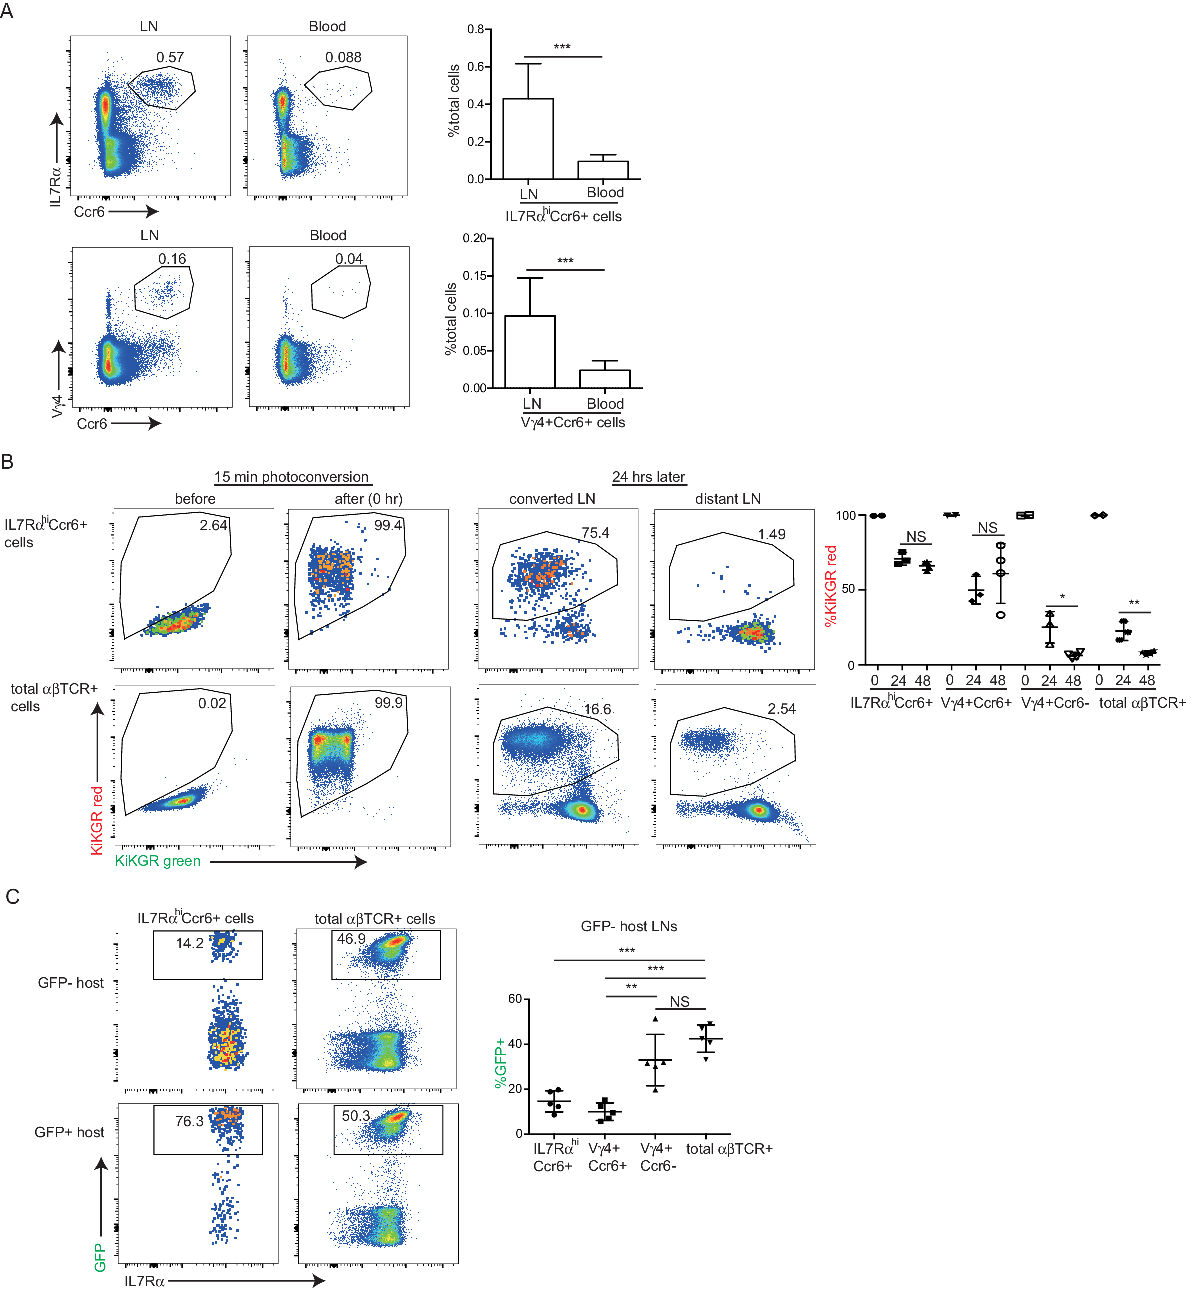
\includegraphics[width=0.95\linewidth]{elife-18156-fig2}
\caption{A very wide figure that takes up the entire page, including the gutter space.}
\label{fig:fullwidth}
\figsupp{There is no limit on the number of Figure Supplements for any one primary figure. Each figure supplement should be clearly labeled, Figure 1--Figure Supplement 1, Figure 1--Figure Supplement 2, Figure 2--Figure Supplement 1 and so on, and have a short title (and optional legend). Figure Supplements should be referred to in the legend of the associated primary figure, and should also be listed at the end of the article text file.}{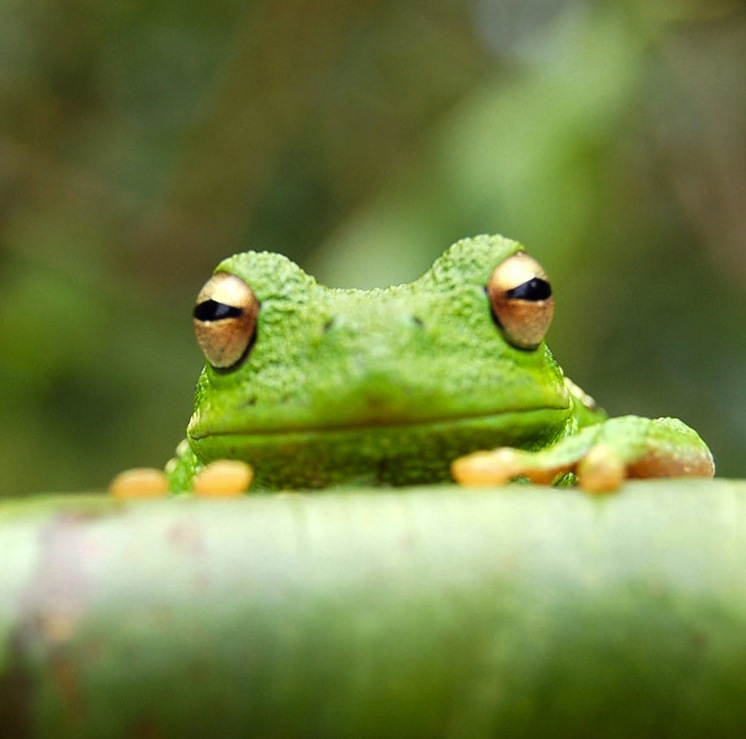
\includegraphics[width=6cm]{frog}}
\end{figure*}


\subsection{Algorithms and Pseudocode}

The \texttt{algpseudocode} and \texttt{algorithms} packages is loaded by the document class. \ALG{euclid} was taken directly from the package documentation. (Please do not load \texttt{algorithm2e}; it's not compatible with \texttt{algpseudocde} nor \texttt{algorithms}!)

\begin{algorithm}
\caption{Euclid's algorithm}\label{alg:euclid}
\begin{algorithmic}%[1]  %% uncomment to enable line numbers
\Procedure{Euclid}{$a,b$}\Comment{The g.c.d. of a and b}
   \State $r\gets a\bmod b$
   \While{$r\not=0$}\Comment{We have the answer if r is 0}
      \State $a\gets b$
      \State $b\gets r$
      \State $r\gets a\bmod b$
   \EndWhile\label{euclidendwhile}
   \State \textbf{return} $b$\Comment{The gcd is b}
\EndProcedure
\end{algorithmic}
\end{algorithm}


\subsection{Citations}

LaTeX formats citations and references automatically using the bibliography records in your .bib file, which you can edit via the project menu. Use the \verb|\cite| command for an inline citation, like \cite{McQuilton01012012}, and the \verb|\citep| command for a citation in parentheses \citep{Aivazian917}. The LaTeX template uses a slightly-modified Vancouver bibliography style.

\begin{featurebox}
\caption{This is an example feature box}
\label{box:simple}
This is a feature box. It floats!
\medskip

\includegraphics[width=5cm]{example-image}
\featurefig{`Figure' and `table' captions in feature boxes should be entered with \texttt{\textbackslash featurefig} and \texttt{\textbackslash featuretable}. They're not really floats.}

\lipsum[1]
\end{featurebox}

\subsection{Mathematics}

\LaTeX{} is great at typesetting mathematics. Let $X_1, X_2, \ldots, X_n$ be a sequence of independent and identically distributed random variables with $\text{E}[X_i] = \mu$ and $\text{Var}[X_i] = \sigma^2 < \infty$, and let
\begin{equation}
\label{eq:CLT}
S_n = \frac{X_1 + X_2 + \cdots + X_n}{n}
      = \frac{1}{n}\sum_{i}^{n} X_i
\end{equation}
denote their mean. Then as $n$ approaches infinity, the random variables $\sqrt{n}(S_n - \mu)$ converge in distribution to a normal $\mathcal{N}(0, \sigma^2)$.

\lipsum[3]

\begin{figure}[hbt!]
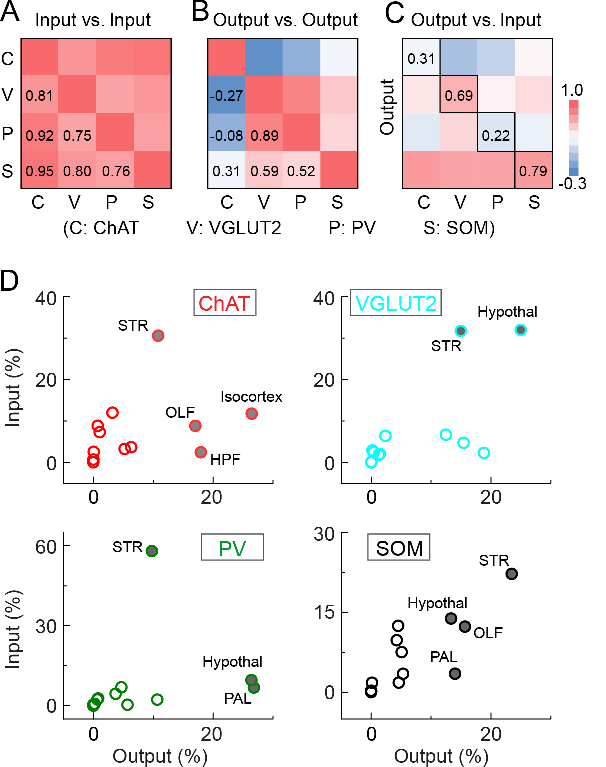
\includegraphics[width=\linewidth]{elife-13214-fig7}
\caption{A column-width example.}
\label{fig:view}
%% If the optional argument in the square brackets is ``none'', then the caption *will not appear in the main figure at all* and only the full caption will appear under the supplementary figure at the end of the manuscript.
\figsupp[Shorter caption for main text.]{This is a supplementary figure's full caption, which will be used at the end of the manuscript.}{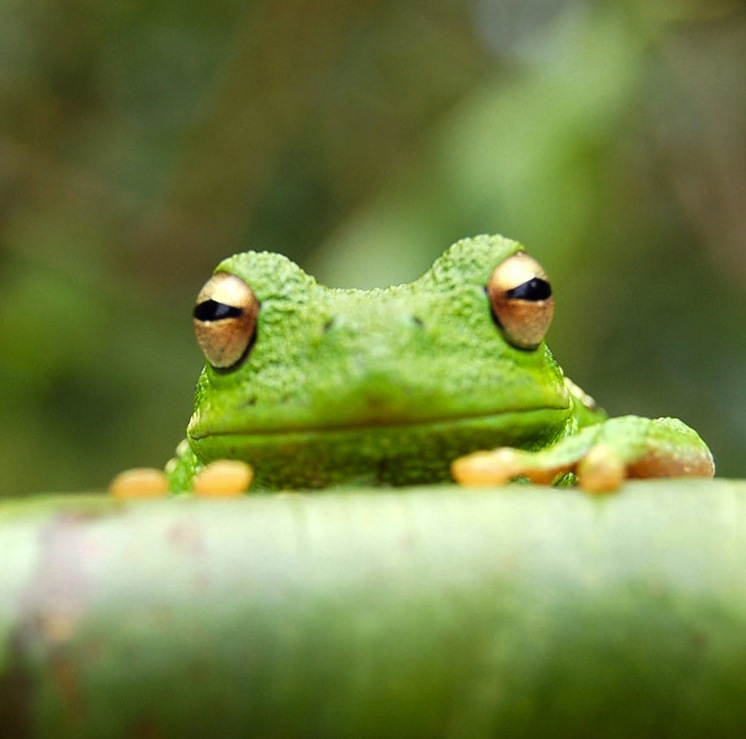
\includegraphics[width=6cm]{frog}}
\figsupp{This is another supplementary figure.}{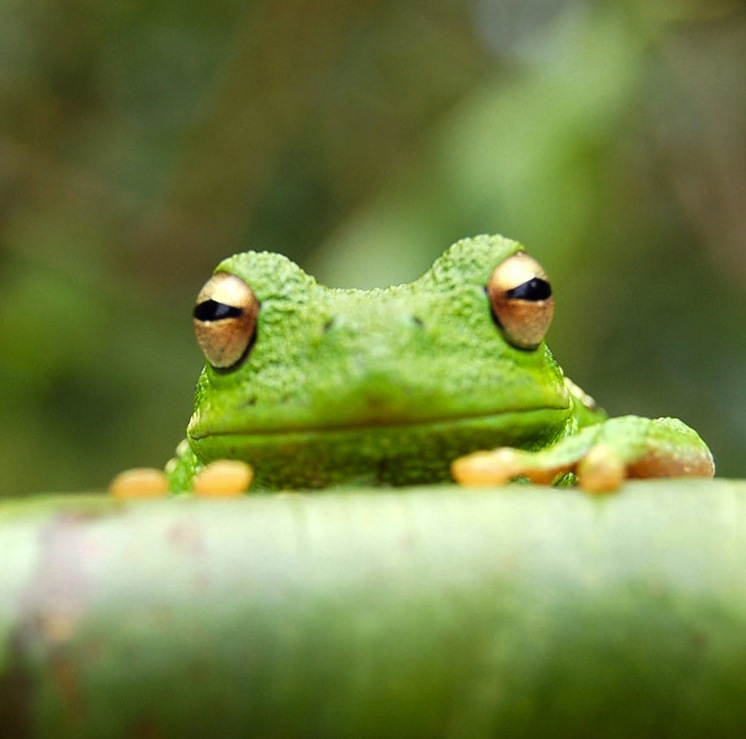
\includegraphics[width=6cm]{frog}}
\figdata{This is a description of a data source.}
\figdata{This is another description of a data source.}
\end{figure}

\subsection{Other Chemistry Niceties}

You can use commands from the \texttt{mhchem} and \texttt{siunitx} packages. For example: \ce{C32H64NO7S}; \SI{5}{\micro\metre}; \SI{30}{\degreeCelsius}; \SI{5e-17}{\Molar}

\subsection{Lists}

You can make lists with automatic numbering \dots

\begin{enumerate}
\item Like this,
\item and like this.
\end{enumerate}
\dots or bullet points \dots
\begin{itemize}
\item Like this,
\item and like this.
\end{itemize}
\dots or with words and descriptions \dots
\begin{description}
\item[Word] Definition
\item[Concept] Explanation
\item[Idea] Text
\end{description}

Some filler text, because empty templates look really poor. \lipsum[1]

\section{Author Contributions}
%%%%%%%%%%%%%%%%
% This section mustt describe the actual contributions of
% author. Since this is an electronic-only journal, there is
% no length limit when you describe the authors' contributions,
% so we recommend describing what they actually did rather than
% simply categorizing them in a small number of
% predefined roles as might be done in other journals.
%
% See the policies ``Policies on Authorship'' section of https://livecoms.github.io
% for more information on deciding on authorship and author order.
%%%%%%%%%%%%%%%%
FMS wrote sections X and Z. RMS contributed to the writing of sections
Y and W.  TMP contributed to the writing of sections Y and W. ITP
contributed to all sections.  ADP wrote sections W and Y, performed
and analyzed the experiments in Z, made figures 4-6, and edited the
whole manuscript as well as standardizing table formatting.
For a more detailed description of contributions,
see the GitHub issue tracking and changelog at \githubrepository.

\section{Other Contributions}
%%%%%%%%%%%%%%%
% You should include all people who have filed issues that were
% accepted into the paper, or that upon discussion altered what was in the paper.
% Multiple significant contributions might mean that the contributor
% should be moved to authorship at the discretion of the a
%
% See the policies ``Policies on Authorship'' section of https://livecoms.github.io for
% more information on deciding on authorship and author order.
%%%%%%%%%%%%%%%
EGP provided inportant insights on the challenges faced by nonequilibrium simulations.
FTP provided several key citations on energy conservation. For a more detailed description of contributions,
see the GitHub issue tracking and changelog at \githubrepository.

\section{Potentially Conflicting Interests}
%%%%%%%
%Declare any competing financial interests.
%%%%%%%
EGP has a 40\% equity stake in the ReallyGoodSimulations company, which sells molecular dynamics code.
DMD is a developer of the package EvenBetterMD, which is recommended in this article.

\section{Funding Information}
%%%%%%%
% Authors should acknowledge funding sources here. Reference specific grants.
%%%%%%%
FMS acknowledges the support of NSF grant CHE-1111111.

\nocite{*} % This command displays all refs in the bib file
\bibliography{livecoms-sample}

%%%%%%%%%%%%%%%%%%%%%%%%%%%%%%%%%%%%%%%%%%%%%%%%%%%%%%%%%%%%
%%% APPENDICES
%%%%%%%%%%%%%%%%%%%%%%%%%%%%%%%%%%%%%%%%%%%%%%%%%%%%%%%%%%%%

\appendix

\section{Firstly}\label{first:app}
\lipsum[1]

\begin{figure}[bt!]
\centering
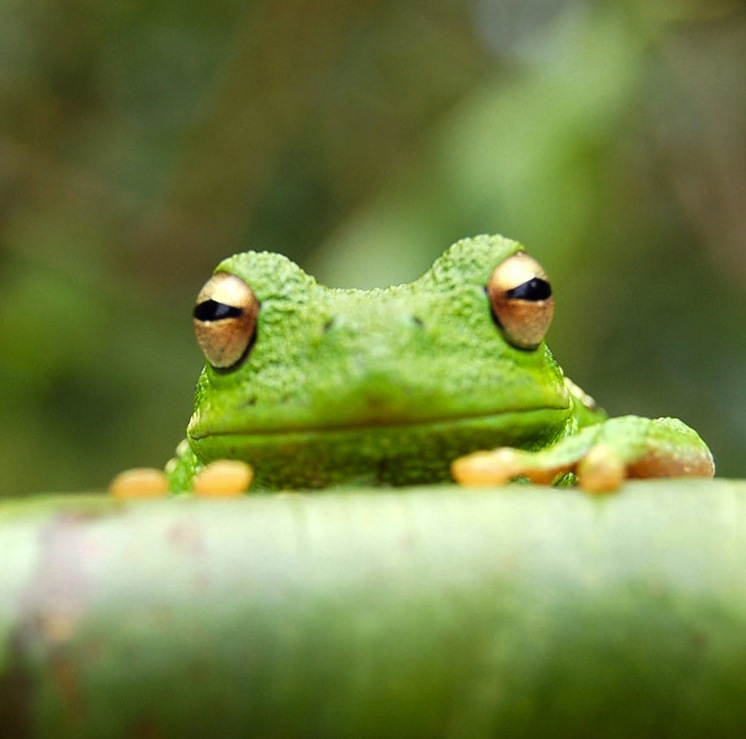
\includegraphics[width=\linewidth,height=5cm]{frog}
\caption{This is a figure in the appendix}
\label{fig:app}
\end{figure}

\section{Secondly}

\lipsum[5-8]

\begin{figure}[hbt!]
\centering
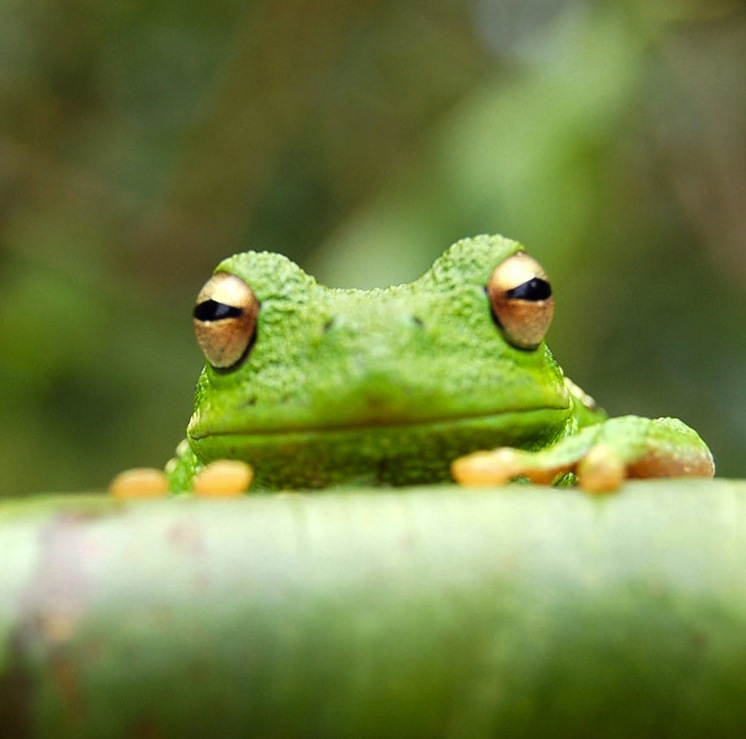
\includegraphics[width=\linewidth,height=5cm]{frog}
\caption{This is a figure in the appendix}
\end{figure}

\begin{figure}[hbt!]
\centering
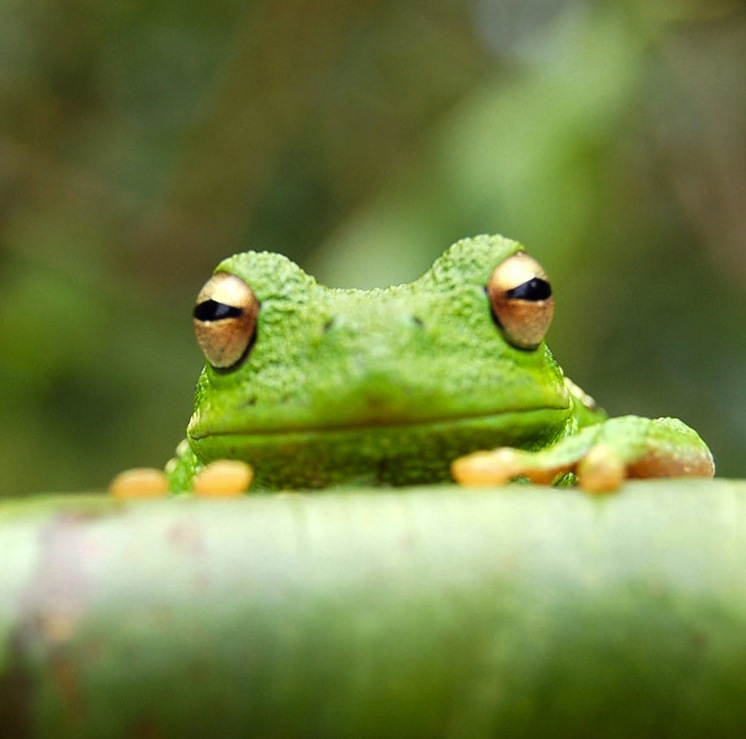
\includegraphics[width=\linewidth,height=7cm]{frog}
\caption{This is a figure in the appendix}
\end{figure}

\end{document}
